\documentclass[11pt,letterpaper,oneside]{book}
\usepackage[parfill]{parskip}
\usepackage{latexsym,fixltx2e}
\usepackage{amsfonts,amsmath,amssymb,siunitx,xcolor,titlesec,blindtext}
\usepackage{chemfig}
\usepackage[version=3]{mhchem}
\usepackage{url}
\usepackage[utf8]{inputenc}
\usepackage{textcomp,notoccite}
\usepackage{multirow,booktabs,appendix}
\usepackage{graphicx}
\usepackage[bf, small, centerlast]{caption}
\usepackage{framed}
\definecolor{shadecolor}{rgb}{0.97,0.97,0.97}
\setlength{\captionmargin}{8pt}
\setlength{\belowcaptionskip}{0pt}

\usepackage[numbers,sort&compress]{natbib}
\usepackage[margin=1.2in]{geometry}

\usepackage{fancyhdr}
\pagestyle{fancy}
\setlength{\headheight}{25pt}
\lhead{Clinton Noack}
\chead{REE Measurement and Recovery}
\rhead{Ph.D. Proposal}

%\usepackage[Lenny]{fncychap}
%\ChTitleVar{\Huge\sffamily\bfseries}

\newcommand{\hsp}{\hspace{10pt}}

\titleformat{\chapter}[hang]{\huge\bfseries}{\thechapter.0\hsp}{0pt}{\huge\bfseries}

\renewcommand{\bibname}{References}
%\newenvironment{codechunk}
%	{\begin{snugshade}
%	 \begin{verbatim}}
%	{\end{verbatim}
%	 \end{snugshade}}

\usepackage{hyperref}

\begin{document}

\frontmatter

%Title page
% Title page. Following CIT formatting.
\thispagestyle{empty}
\begin{center}

\Huge{\textbf{Measurement and Recovery of Rare Earth Elements from Hypersaline Fluids}}
\vspace{1cm}

\normalsize{Ph.D. proposal update}
\vspace{1cm}

\Large{Clinton W. Noack}
\vspace{1cm}

\normalsize{
Department of Civil and Environmental Engineering

Carnegie Mellon University

Pittsburgh, PA 15213}
\vspace{2cm}

\normalsize{
\textbf{Ph.D. Committee and affiliations}

Professor Athanasios Karamalidis (co-advisor), CEE

Professor David Dzombak (co-advisor), CEE

Dr. J. Alexandra Hakala, NETL-Pittsburgh

Professor Mitchell Small, CEE

Professor Newell Washburn, Chemistry
}

\vspace{1cm}


4 November 2015

\end{center}

 \clearpage

\chapter{Abstract}
The rare earth elements (REE) are a suite of 16 elements with coherent and predictable chemistries with ubiquitous utilization in modern technology.
While not truly rare in average abundance, the lack of concentrated deposits and the challeneges of intra-group separations make these elements highly valuable and difficult to produce in mass.
Large economic and environmental costs associated with primary REE extraction motive the development of alternative REE resources, such as concentrated brines.
This thesis will focus on the occurrence of REE in hypersaline fluids and the separation of the REE from these fluids.

The development of the Marcellus shale for natural gas provides an excellent case study for the use of REE in source identification and apportionment.
Both the character (i.e. elevated salinity, dissolved heavy metals, naturally occurring radioactive material) and volume (millions of liters per drilled well) of waste brines associated with the oil and gas extractive industry provide sufficient motivation for investigation of advanced monitoring tools for protection of freshwater resources.
Similarly, the wide variety of contaminant sources (i.e. having the potential to degrade high quality waters) in Southwestern Pennsylvania --- including conventional oil and gas wastewater, abandoned mine drainage, varied industrial wastes, municipal waste, and agricultural run-off --- further promote the search for analytes which would allow for discrimination among potential sources.

The REE have previously been used to hypothesize groundwater mixing and sources of salinity in steady-state systems.
However, these methods have either lacked mathematical rigor (i.e. are qualitative and typically based on visual inspection of REE profiles) or have failed to consider variability in source signatures while assuming conservative behavior (i.e. deterministic).

The goals of this research will be to evaluate the feasibility of using REE as tracers of saline groundwaters, and to determine the appropriate mathematical and statistical models for interpreting REE data for environmental forensics.
The development of these models will be supported through focused experimentation and development of analytical techniques along with consideration of previously published data and adaptation of existing source apportionment models.

The goals of the research will be achieved through four specific objectives.
The first objective of this work will be to accumulate available water quality data with REE measurements from the literature and explore relationships among the REE as well as between the REE and other commonly measured, bulk analytes.
The second objective will be to develop and validate an efficient liquid-liquid extraction for determination of REE in hypersaline brines.
The third objective will be to study the effects of ligand functionality and geometry on the partitioning behavior of the REE from brines to functionalized adsorbents.
The final objective will be to study the best performing adsorbent(s) in detail.
Taken together, these objectives will be a contribution to the understanding of trace-metal geochemistry, particularly in high salinity systems, and an assessment of extraction and recovery strategies targeted at the REE in hypersaline fluids.

\tableofcontents

\listoffigures
\addcontentsline{toc}{chapter}{List of Figures}

% Chapter 1 - Intro, problem, goals
\mainmatter

% Introduction
\chapter{Introduction}
\vspace{-1cm}

Modern technologies --- including catalysts, high-strength alloys, high-efficiency phosphors, lasers, and magnets --- are dependent upon the unique properties of the rare earth elements (REE) for their efficacy of operation.
However, global REE material-flows are prone to complex environmental, technical, and geopolitical forces on both the supply- and demand side.
Development of economically-viable technologies for the extraction of the REE and other critical materials from unconventional sources (such as geothermal fluids, oil and gas produced waters, or coal combustion residuals) has great potential value to: generate a consistent domestic supply of materials critical to green energy and defense technologies; valorize high-volume wastes or low-value industrial byproducts; and avoid environmental impacts from primary REE mining.

\section{What are rare earth elements?}
The REE constitute much of Group 3 of the periodic table, a group of 16 transition metals, including the lanthanide series (La to Lu, excluding Pm), Yttrium (Y) and Scandium (Sc).
The ``rare'' moniker stems from their initial isolation from uncommon mineral phases in the 18th and 19th century \citep{CastorHedrick},
though the natural abundance of REE in the earth's crust range from 0.52 parts per million (ppm) to 41.5 ppm, in the same range as Pb or Sn and exceeding the natural, crustal abundance of Ag and Hg \citep{CRC}.

In the natural sciences, predictable thermodynamic differences between the REE make these elements uniquely capable tools for interpreting natural geologic and chemical processes \citep{Murray_Geol_1990, Laveuf_Geoderma_2009}.
Rare earth lithogeochemistries have long been used to infer depositional environments of geologic strata \citep{Murray_Geol_1990, PAAS, Hanson_AREPS_1980}.
Similarly, REE serve as benign analogs to the transuranic actinide series for nuclear waste disposal studies \citep{Krauskopf_CG_1986, Millero_GCA_1992};
as potential markers of regional authenticity for high value exported food products such as wine, pumpkin-seed oil, and olive oil \citep{Jakubowski_FJAC_1999, Joebstl_FC_2010, Farmaki_AL_2012};
and for studying mixing and metal cycling in the oceans \citep{DeBaar_Nature_1983, Elderfield_PTRS_1988}.

Many of the same properties that yield the unique and predictable geochemistry of the REE have lead to their use in more consumer products than nearly any other element group \citep{CastorHedrick, Graedel_PNAS_2015}. In most applications, the performance of the REE is unmatched \citep{Ciacci_EST_2015, Nassar_JIE_2015}, making substitution (with more readily available/environmentally benign elements) undesirable.

Based on atomic number, the REE are segregated into light and heavy REE (LREE and HREE, respectively) with the division occurring between Eu and Gd \citep{CastorHedrick};
some studies further distinguish middle REE (MREE), though the specific elements are inconsistently defined between authors \citep{Hannigan_CG_2001, Tang_CG_2010, Choi_CG_2009}.
These ``weight'' distinctions allow for simplified description and quantification of the inter-element relationships, typically ratios of normalized concentrations, which are exploited in REE analysis.
Similarly, anomalies of certain REE --- due to redox lability for Ce and Eu \citep{Brookins_RMG_1989} and large anthropogenic emissions for Gd \citep{Bau_EPSL_1996} --- are used to interpret geochemical processes.
Y and Sc exhibit similar properties to the lanthanides and are thus included in the suite of REE with Y being most similar to HREE and Sc being most similar to LREE in solution \citep{Brookins_RMG_1989}. 

\section{What is the context of this study?}

The constantly increasing consumer products incorporating the REE, and the ensuing demand for these products, have established the REE as valuable global commodities.
Domestic demand in 2012 was 11,300 tons, while the global demand was more than 113,000 tons \citep{FrostSullivan_REEmarket}.
Much of that demand is a result of a booming green energies market.
In particular, the permanent magnets sector is expected to experience significant growth between 2013 and 2020.
High-efficiency generators used in turbines and electric motors require strong and light permanent magnets.
Currently, magnets using neodymium, praseodymium, and samarium (with dysprosium and terbium additives) are the strongest and lightest commercially available.

Even at the height of domestic REE production at Mountain Pass in CA (2012), the U.S. imported \$520MM worth of REE compounds, with nearly 40\% coming from China, in order to support a demand of 11,300 tons \citep{USGS_minyb_2012}.
A booming green energies industry fueled, and continues to fuel, both domestic and global demand, where the REE provide superior performance and efficiency compared to alternative materials \citep{Nassar_JIE_2015, Graedel_PNAS_2015}.
Sustained growth in these technologies is dependent on diversifying REE sources given projected supply shortages in the medium- to long-term.
Traditional mining of REE from ore deposits is unlikely to fulfill this demand for technical and economic reasons, especially in the US where traditional mining of REE is suspended.
China, the world's leading source of REE and primary supplier of global demand for many years (Figure~\ref{fig:world-REO-prod}, has indicated partial control of exports, or punitive tariffs, in the near future.
This emphasizes the need for REE separation and recovery from unconventional matrices, such as geothermal fluids or coal fly ash.

\begin{figure}[htbp]
\begin{center}
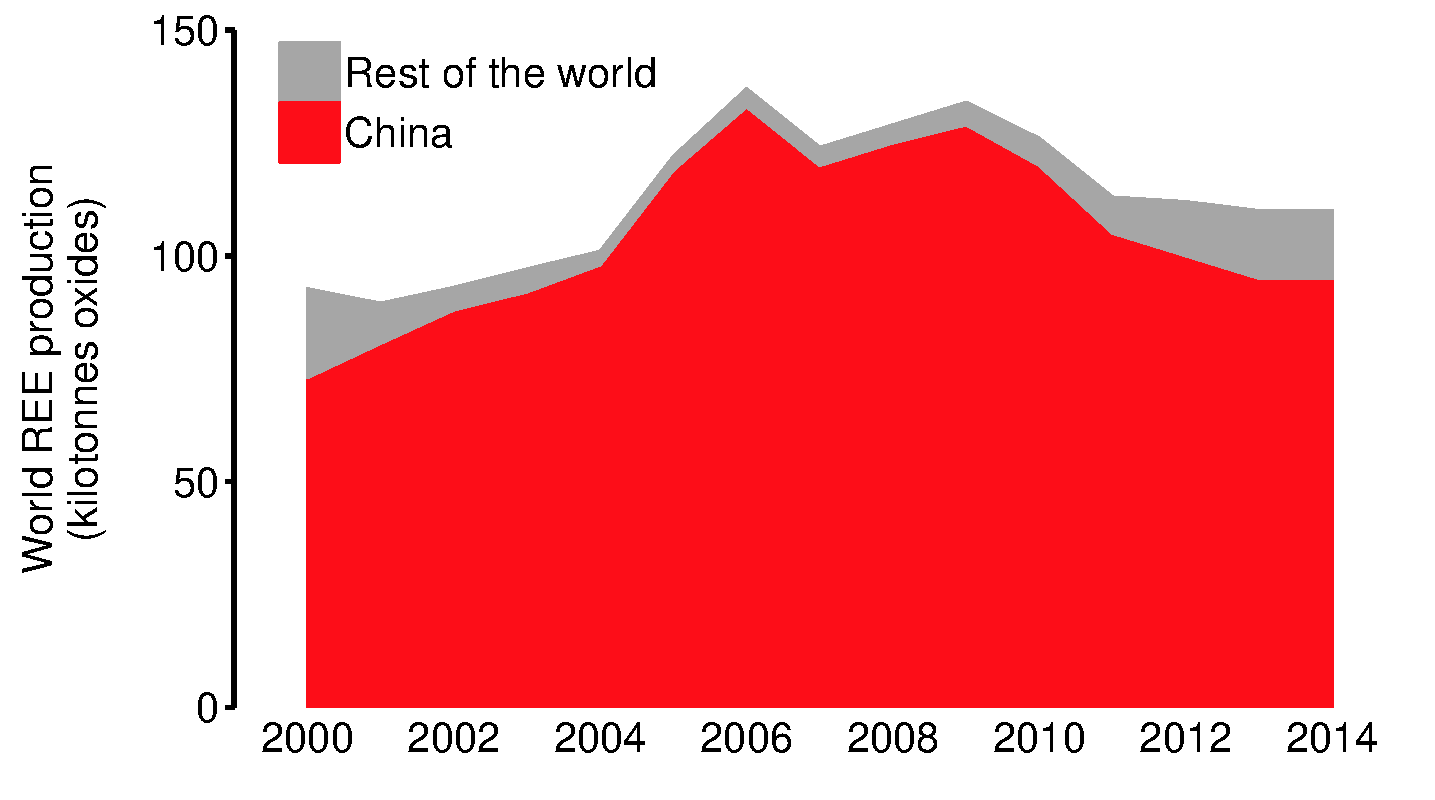
\includegraphics[width = 0.7\textwidth]{proposal_figures/World-REO-production.pdf}
\caption{Global, primary REE production, 2000-2014.
Data from \citet{USGS_commsumm}.}\label{fig:world-REO-prod}
\end{center}
\end{figure}

Global REE reserves are estimated at 130 million metric tons \citep{USGS_commsumm}, much of which is located in low-concentration deposits or ocean-floor manganese nodules, which are both extremely expensive to mine with current methods.
This limits the number of readily mineable REE deposits and, ultimately, our ability to increase REE supply \citep{JRC_2011, Alonso_EST_2012}.
Aqueous media such as brines or produced waters from geothermal energy, conventional oil/gas, and shale gas extraction operations are potentially significant, but unexplored sources of REE.

Presently, REE extraction is accomplished by traditional mining (e.g. open-pit) followed by chemically-, and energy-intensive element separations, which incur a significant environmental burden (Figure~\ref{fig:Zaimes-LCA}; \citep{Zaimes_SCE_2015}).
Even when present in ores at appreciable levels, REE are commonly commingled with radioactive thorium and uranium, which need to be safely separated and stored in addition to standard waste management associated with mining (e.g. tailings) \citep{Gupta_IMR_1992, Sprecher_EST_2014}.
Stringent environmental regulations, time-intensive processes, and expensive permits complicate the opening of new, domestic mines because of these inherent risks.
On this basis, projections expect that exploiting traditional REE sources to meet increasing demand will be a significant challenge.
In 2012, China was responsible for more than 95\% of the global REE supply \citep{USGS_commsumm}.
China also had the largest demand for REE, at 66\% of the total global demand \citep{USGS_commsumm}.
The US was the next largest consumer, at 10--15\% of the total demand.
In 2011, China announced a 35\% reduction in exports of REE, in an effort to meet their domestic needs \citep{USGS_minyb_2012}.
This created large instability in the REE market as there were no other major sources for REE \citep{Alonso_EST_2012, Chakmour_Elem_2012, Hatch_Elem_2012}.
China is expected to continue reduction of exports, through either quotas or tariffs, as a mean to reduce stress on its REE reserves \citep{FrostSullivan_REEmarket, USGS_commsumm}.

\begin{figure}[htbp]
\begin{center}
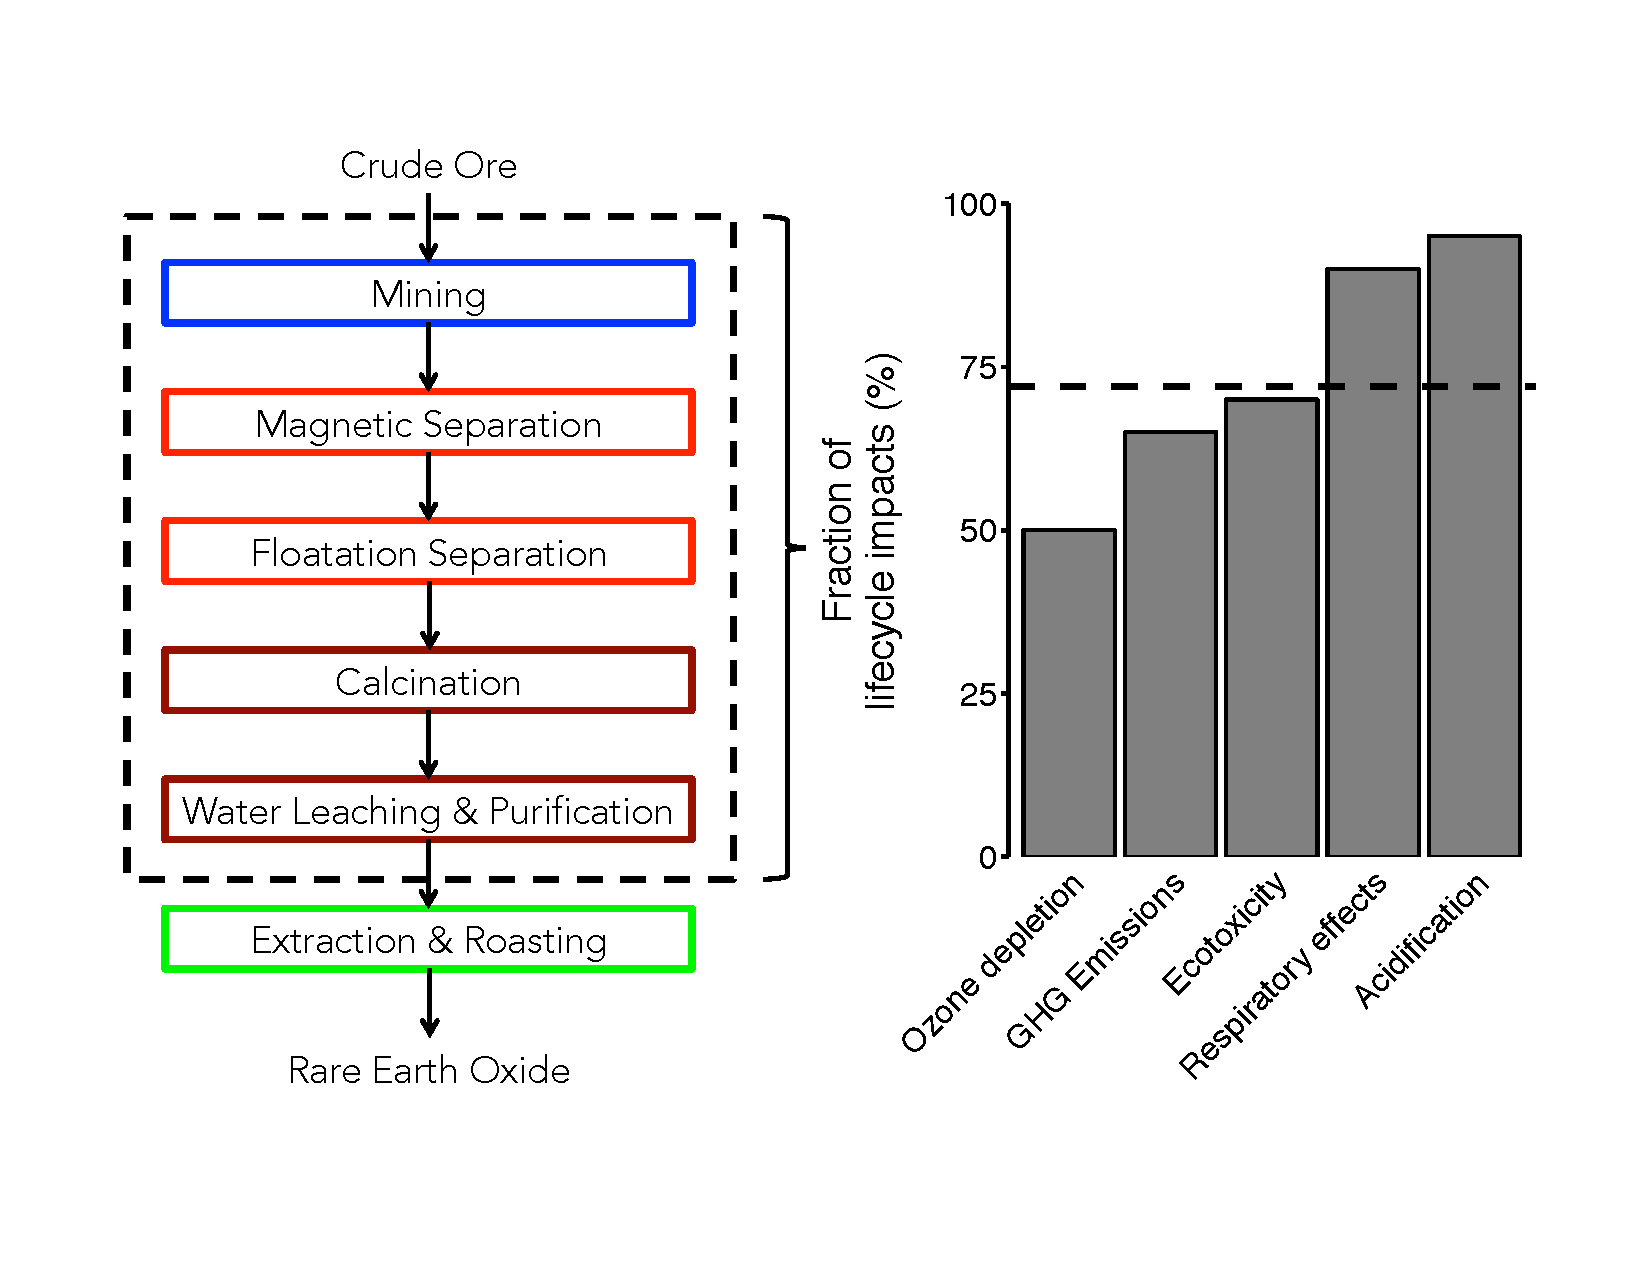
\includegraphics[width = \textwidth]{proposal_figures/Zaimes-LCA-schematic.pdf}
\caption{Traditional REE production flowsheet (left) and the associated fraction of lifecycle environmental impacts for the boxed boundary (right) using data from \citet{Zaimes_SCE_2015}.
Only selected impact categories are shown, however the dashed line (72\%) indicates the overall average across ten categories.}\label{fig:Zaimes-LCA}
\end{center}
\end{figure}

Primary mining effectively constitutes 100\% of the REE production worldwide \citep{Binnemans_JCP_2013, USGS_commsumm},
but interest in recovery of REE from end-of-life stocks (EOL), from unconventional resources, and from REE-containing industrial wastes has expanded rapidly in recent years \citep{Binnemans_JCP_2015}.
High volumes of REE are deployed in permanent magnets, while high-value REE are used in phosphors \citep{Hatch_Elem_2012},
making these products two primary targets for recycling from EOL products along with metal hydride batteries \citep{Binnemans_JCP_2013,Tunsu_Hydro_2015}.
REE are applied in many other products, but the REE content is dissipated in-use or rendered unrecyclable by current designs \citep{Ciacci_EST_2015}.
Ferrous shredder waste (where magnets could accumulate) is a promising potential resource for REE and other critical materials.
However, \citet{Bandara_JSM_2015} propose that recycling of ferrous shredder-waste would need to exceed 50\% in order to dampen Nd price volatility from recycling alone. The conclusion from these forecasts is the need for novel, alternative feedstocks \citep{Bandara_JSM_2015}.

\section{What are the goals of this study?}
This research seeks to address the potential for REE extraction and recovery from dilute aqueous sources.
This work is motivated by the desire to diversify REE sources, promote development of low-carbon energy sources, valorize industrial byproducts, and avoid the environmental disruption associated with primary REE mining.
A combination of a literature analysis, analytical method development, controlled experimentation, and statistical and geochemical modeling will be used to address these goals.

The three, specific objectives of this work and the related questions they were developed to answer are as follows:
\begin{enumerate}
	\item Determine REE abundance and trends in natural waters.
	\begin{itemize}
		\item	What is the natural variability of REE in aqueous media?
		\item	What quantitative methods exist for considering below detection limit values?
		\item	What is known about REE occurrence in brines?
		\item	What relationships between REE and bulk solution properties are important for REE fate and transport?
	\end{itemize}
	\item Develop efficient liquid-liquid extraction technique for separation of REE from hypersaline brines.
	\begin{itemize}
		\item	How are REE measured in aqueous samples?
		\item Will these techniques work for hypersaline, chemically complex brines?
		\item What are the limits of effectiveness for an LLE technique (with respect to brine composition)?
	\end{itemize}
	\item	Study the effects of ligand functionality and geometry on the partitioning behavior of the REE from brines to functionalized adsorbents
	\begin{itemize}
		\item	What ligands have high, aqueous-phase affinity for the REE?
		\item How does surface attachment affect the affinity of these ligands for the REE?
		\item What are the best performing ligands for REE recovery?
		\item How do these ligands perform under a range of aqueous conditions? 
	\end{itemize}
\end{enumerate}

The specific objectives of this work were developed to address gaps in the literature to date while building on the existing REE and functionalized adsorbent knowledge base. These objectives are meant to address application specific (i.e. REE recovery from geothermal brines) uncertainty as well as foster a more fundamental understanding of the REE systematics. The methods proposed to address these objectives are detailed in \S2.1-2.3.


% Introduction
\chapter{Research plan}
\vspace{-1cm}

Four specific objectives were developed for this work, combining literature review, data analysis, analytical technique development, focused experimentation, and modeling:

\begin{itemize}
	\item Determine REE abundance and trends in natural waters.
	\item	Develop efficient liquid-liquid extraction technique for separation of REE from hypersaline brines
	\item Study the effects of ligand functionality and geometry on the partitioning behavior of the REE from brines to functionalized adsorbents
\end{itemize}

These individual tasks are described subsequently in \S 2.1--2.4.

\section{Determine REE abundance and trends in natural waters}

In this objective, a compilation and analysis of data from numerous independent studies of REE in natural waters was performed.
The compiled data were used to develop a consistent database of REE concentrations and their associated major solute chemistry and to explore interelement relationships, examine trends in REE abundance, and test hypotheses related to REE abundance as functions of major solution chemistry parameters.
The tasks within this objective were: (1) to ascertain an expected range of dissolved REE concentrations in waters of variable chemistries, (2) to derive unbiased estimates of REE distributions, and (3) to investigate trends in REE abundance in groundwater in relation to other available chemical parameters (e.g. pH, ionic strength, and major solution species).
Results of this work have been published and described in detail in Noack, et al.50 which is included in Appendix A.1.

The major findings of this work were that the REE are found in natural waters across ten orders of magnitude of concentrations, that pH appears to be the only variable at the ``macro'' scale of this study which significantly influences abundance, and that, while limited data exist for REE in brines, the REE composition of brines is potentially unique.
These results have implications on the remainder of this project.
First, the natural variability and lack of data of REE in brines necessitates development of robust, reliable analytical techniques for such waters as well as the application of this technique to hypersaline brine samples.
Second, the lack of consistent predictors of REE abundance requires focused experimentation of REE source and sink behavior in the environments of interest.

\section{Develop a liquid-liquid extraction technique for separation and concentration of REE from brines}

In this objective, REE separation and preconcentration from highly saline brines using a liquid-liquid method was studied.
A significant limitation of published methodologies for REE quantification in aqueous samples is the lack of validation of the methods in systems with high salinity and dissolved metals.
A common ligand used for REE complexation and extraction, bis(2-ethylhexyl) phosphate (HDEHP), was studied in a heptane diluent. 
The tasks of this objective were to: (1) demonstrate feasibility of REE recovery from small volumes of hypersaline brines by LLE, (2) optimize LLE methodology for high salinity and metals content, and (3) validate method for synthetic brines of varying complexity.
Results of this work have been published and described in detail in Noack, et al.50 which is included in Appendix A.2.

The major finding of this work was that the REE are measurable at environmentally relevant concentrations in hypersaline solutions with high accuracy using small volumes of samples.
Moreover, the method is robust to variability in salt, dissolved organic carbon, and competing metal concentrations.
This method can be confidently applied to the analysis of natural samples in the future for calibration of engineered recovery systems.

\section{Study REE partitioning to novel functionalized adsorbents from saline solutions}

% Expected contributions and broader impacts
\chapter{Major contributions and broader impacts}
\vspace{-1cm}

At the conclusion of this research, we expect to have contributed significant knowledge to the field of REE geochemistry, in particular, as it applies to saline fluids.
While the context of this work primarily relates to geothermal waters, the potential for extraction of REE from aqueous media is far reaching.
Other large-scale engineering processes such as carbon capture, utilization, and storage (CCUS), desalination waste-brine management, or oil and gas production handle large volumes of highly saline waters that may contain valuable quantities of REE.
Moreover, highly selective adsorbents would represent a significant improvement compared to the relatively non-specific ligands utilized in solvent extractions during traditional REE production schemes.

More specifically, each objective of this research is expected to improve understanding of REE geochemistry.
In Objective 1, the compilation and analysis of literature data highlighted the enormous variability in dissolved REE concentrations, while identifying the lack of knowledge regarding the controls on REE abundance and the occurrence of REE in hypersaline solutions.
Objective 2 will provide a robust and rigorously validated technique for filling in this gap, allowing for reliable determination of the REE in brines, without requiring large sample volumes.
Finally, Objective 3 provides systematic study of the effects of surface attachment of ligands, with known aqueous REE affinity, for use in an extraction and recovery scheme.
As yet, economically viable alternatives to traditional REE extraction are almost non-existent.
This work represents the early stages of developing a technology with the potential to generate a consistent domestic supply of materials critical to green energy and defense technologies; valorize high-volume wastes or low-value industrial byproducts; and avoid environmental impacts from primary REE mining..


\begin{appendix}

%\chapter{Supporting information for Chapter~\ref{chap:REE-review}}
\chaptermark{SI for REE in natural waters}
\section{Weighted Kaplan-Meier estimation of survival function for analyzing left-censored data}
\sectionmark{Analysis of left-censored data}

The weighted Kaplan-Meier (KM) estimator (\(\widehat{S}(x_i)\)) is expressed as:

\begin{align*}
\widehat{S}(x_i) = \prod_{x \geq x_i}\left(1 - \frac{d_i^w}{Y_i^w}\right)
\end{align*}

where, for application to aqueous chemistry data, \(\widehat{S}(x_i)\) is estimate of the probability of any measured concentration, \(x\), from the population being \emph{less} than \(x_i\).
It is calculated using the weighted count of uncensored observations at \(x_i\) (\(d_i\)) and the weighted count of all (censored or uncensored) observed concentrations less than \(x_i\) (\(Y_i^w\)).
The weighting of each data point is calculated here as the inverse of the number of samples from the data source, or \(w_i = n_i^{-1}\).
This curve can be used to estimate the quantiles of the data distribution as well as make estimates of the mean and variance of the population.
The computational methods here are adapted from Xie and Liu \citep{Xie_SiM_2005} and Singh et al. \citep{Singh_JAWMA_2013}.

To demonstrate these calculations, random data, drawn from log-normal distributions, will be used, followed by analysis of the groundwater REE dataset.
This analysis makes use of functions from the \texttt{plyr} (V 1.8.1), \texttt{dplyr} (V 0.3.0.2), and \texttt{tidyr} (V 0.1) packages which must be installed to run this analysis.
Aside from the pipe operator (\texttt{\%\textgreater{}\%}, loaded via the \texttt{dplyr} namespace, but part of the \texttt{magrittr} package), functions from these namespace are denoted as \texttt{package\_name::function\_name}, e.g. \texttt{dplyr::mutate}. 

Code, written in R, is shown with a grey-shaded background:

\begin{snugshade}
\begin{verbatim}
# This is an R comment
X <- 10
Y <- rnorm(1000)
\end{verbatim}
\end{snugshade}

Conversely, output from R calculations will be shown as:

\begin{verbatim}
##
## These are results
##
\end{verbatim}

\subsection{Generation of random data}
% Width of page (do not let code extend beyond)
% --------------------------------------------------------------------------------
\begin{snugshade}
\begin{verbatim}
## If these packages are not installed,
## un-comment and run these lines
# install.packages('plyr')
# install.packages('dplyr')
# install.packages('tidyr')
library(plyr)
library(dplyr)

# Data are drawn from three separate log-normal distributions
# Group means
means <- c(1,1.5,2.5)

# Samples in each group
N <- 100

# Generate random data
set.seed(8675309)
R <- data.frame(sapply(means, function(mu) rlnorm(N, mu, 1)))
colnames(R) <- c('Grp1','Grp2','Grp3')
head(R) # Look at first few values of random data, R

# `mutate` adds censoring and site ID
R.g <- tidyr::gather(data = R, key = Dataset,
                     value = Concentration,
                     contains('Grp')) %>%
         # Assume that 60% of samples were analyzed by
         # method with DL = 1 ppb, 40% with DL = 10 ppb
  dplyr::mutate(DL = sample(c(1, 10),
                            size = nlevels(Dataset)*N,
                            replace = T,
                            prob = c(0.6,0.4)),
         # Flag censored values and store at detection limit
         Censored = ifelse(test = Concentration < DL,
                           yes = 1, no = 0),
         Concentration = ifelse(Censored == 1,
                                DL, Concentration),
         # Randomly assign to sites w/ non-uniform probability
         Site = sample(LETTERS[1:10],
                       nlevels(Dataset)*N,
                       replace = T,
                       prob = 1:10/sum(1:10))) %>%
  dplyr::select(Dataset, Concentration, Censored, Site)

# Look at first few rows of fictional, partially censored data.
dplyr::tbl_df(R.g)
\end{verbatim}
\end{snugshade}

\begin{verbatim}
## Source: local data frame [300 x 4]
## 
##    Dataset Concentration Censored Site
## 1     Grp1        10.000        1    D
## 2     Grp1        10.000        1    J
## 3     Grp1        10.000        1    I
## 4     Grp1        20.685        0    H
## 5     Grp1         7.889        0    J
## 6     Grp1        10.000        1    I
## 7     Grp1         2.794        0    H
## 8     Grp1        10.000        1    I
## 9     Grp1         4.817        0    G
## 10    Grp1        10.000        1    F
## ..     ...           ...      ...  ...
\end{verbatim}

\subsection{Functions of the weighted Kaplan-Meier routine}

To utilize the weighted KM, the weights of each observation must be calculated.

\begin{snugshade}
\begin{verbatim}
calc_weights <- function(site_vector){
  counts <- data.frame(Site = site_vector) %>%
    dplyr::group_by(Site) %>% 
    dplyr::summarise(weight = 1/n())
  return(counts)
}

# Weights of sites are very similar across groups
# Note that no samples were assigned to "Site" A in Grp3,
# thus the weight is NA
plyr::ddply(R.g, .(Dataset), function(df){
    calc_weights(df$Site)
  }) %>%
  tidyr::spread(Dataset, weight)
\end{verbatim}
\end{snugshade}

\begin{verbatim}
##    Site    Grp1    Grp2    Grp3
## 1     A 0.25000 0.20000      NA
## 2     B 1.00000 0.20000 1.00000
## 3     C 0.16667 0.16667 0.20000
## 4     D 0.14286 0.16667 0.14286
## 5     E 0.25000 0.14286 0.08333
## 6     F 0.08333 0.08333 0.08333
## 7     G 0.12500 0.06667 0.12500
## 8     H 0.05000 0.10000 0.05263
## 9     I 0.06667 0.06667 0.05556
## 10    J 0.04348 0.05263 0.05556
\end{verbatim}

Next, the function for calculating the survival estimator is built.

\begin{snugshade}
\begin{verbatim}
Surv_weighted <- function(censored_data){
  # Data should have the following form [R data type]:
  # Column 1 = `Concentration` [double]
  # Column 2 = `Censored` [bool/int]
  # Column 3 = `Site` [factor]
  
  if(!is.factor(censored_data$Site)){
    censored_data$Site <- factor(censored_data$Site)
  }
  
  # Get weights
  site_weights <- calc_weights(censored_data$Site)
  
  # Combine weights with original data
  data_mod <- dplyr::left_join(censored_data,
                               site_weights,
                               by = 'Site')
  
  # Calculate the `at risk` observations, or
  # weighted # of observations less than each concentration
  data_mod <- dplyr::arrange(data_mod,
                             # Data in descending order
                             desc(Concentration)) %>%
    dplyr::mutate(Yw = sum(weight) - cumsum(weight) + weight)
  
  # Retain only uncensored (Censored == 0) observations
  observed <- dplyr::filter(data_mod, Censored == 0) %>%
    dplyr::select(-Censored)
  
  # All observations with identical values are counted
  obs_weight_tab <- dplyr::group_by(observed, Concentration) %>%
    dplyr::summarize(dw = sum(weight))
  
  # Combine weighted counts with rest of data and calculate S
  observed <- dplyr::left_join(observed, obs_weight_tab,
                               by = "Concentration") %>%
    # "incremental survival", value inside product
    dplyr::mutate(P = 1 - dw/Yw) %>%
    # Remove duplicated observations
    dplyr::filter(!duplicated(Concentration)) %>%
    dplyr:: mutate(S = cumprod(P),
                   S = ifelse(S<0,0,S))
  
  return(observed)
}
\end{verbatim}
\end{snugshade}

Using the simulated data, these functions can be tested:

\begin{snugshade}
\begin{verbatim}
# Calculate weighted KM for each dataset/group
sim_wKM <- R.g %>% plyr::ddply(.(Dataset), function(df){
  df <- dplyr::select(df,-Dataset)
  wKM <- Surv_weighted(df)
  return(wKM)
})

# Look at results
sim_wKM %>% 
  dplyr::select(Dataset, Concentration, weight, S) %>%
  dplyr::tbl_df()
\end{verbatim}
\end{snugshade}

\begin{verbatim}
## Source: local data frame [207 x 4]
## 
##    Dataset Concentration  weight      S
## 1     Grp1        20.685 0.05000 0.9950
## 2     Grp1        20.505 0.16667 0.9783
## 3     Grp1        19.803 0.08333 0.9700
## 4     Grp1        19.540 0.04348 0.9657
## 5     Grp1        14.310 0.06667 0.9590
## 6     Grp1        13.423 0.06667 0.9523
## 7     Grp1        13.130 0.04348 0.9480
## 8     Grp1        11.808 0.08333 0.9396
## 9     Grp1         9.981 0.25000 0.9038
## 10    Grp1         9.503 0.06667 0.8942
## ..     ...           ...     ...    ...
\end{verbatim}

To estimate the quantiles of a dataset with censoring, \texttt{Surv\_quantile} is defined, which calls \texttt{Surv\_weighted}.
This function will choose the observation closest to the desired quantile, without exceeding that quantile.
As in the main text, if the calculated survival quantiles, $S(x)$, for adjacent observations were $S(x_1)=0.94$ and $S(x_2)=0.96$, then $x_1$ would be noted as the 95$^{th}$ percentile.
If the desired quantile is outside of the range of calculated  (e.g. for $Q(0.05)$ when $\min \widehat{S}(x) > 0.05$), the quantile is estimated parametrically through regression on order statistics (ROS).
Here the data are assumed to be adequately fit by a log-normal distribution.
The parameters of this distribution are estimated from quantile-quantile regression.

\begin{snugshade}
\begin{verbatim}
Surv_quantile <- function(censored_data,
                          # Default to median + IQR
                          percentiles = c(0.25,0.5,0.75),
                          sig.fig = 3){
  # Fraction of data below detection
  cenfrac <- mean(as.logical(censored_data$Censored))
  
  # Calculate wKM and select relevant columnes
  weighted_km <- Surv_weighted(censored_data) %>%
    dplyr::select(Concentration, S)
  
  # Warnings about data
  if(any(cenfrac > percentiles)){
    warning(paste('The fraction of censored data is larger ',
                  'than one or more desired percentiles.\n',
                  'This may produce unreliable estimates.',
                  sep = ''))
  }
  
  out_of_range <- c(F,F)
  
  if(any(percentiles < min(weighted_km$S))){
    warning(paste('At least one desired percentile below', 
                  'minimum calculated from data,', 
                  'will be estimated from ROS.'), sep = ' ')
    out_of_range[1] <- T
  }
  
  if(any(percentiles > max(weighted_km$S))){
    warning(paste('At least one desired percentile above', 
                  'maximum calculated from data,', 
                  'will be estimated from ROS.'), sep = ' ')
    out_of_range[2] <- T
  }
  
  if(any(out_of_range)){
    ROS_data <- dplyr::filter(weighted_km, !is.na(S)) %>%
      transmute(y = log(Concentration), x = qnorm(S))
    ROS <- with(ROS_data,
                lm(y ~ x)
                )
    
    # Function for returning predictions based on ROS
    pred_ROS <- function(ROS_obj, percentile){
      new_dat <- data.frame(x = qnorm(percentile))
      log_pred <- predict(ROS_obj, newdata = new_dat)
      return(exp(log_pred))
  }
  
  fl.h <- function(percentile, S){
    h.temp <- which.min(abs(S - percentile))
    return(h.temp)
  }
  
  h.low <- sapply(percentiles, function(p){
      fl.h(p, weighted_km$S)
    })
  perc_df <- data.frame(Percentile = percentiles) %>%  
    dplyr::group_by(Percentile) %>%
    dplyr::mutate(h.low = fl.h(Percentile, weighted_km$S),
                  use_ROS = ifelse(
                    (Percentile < min(weighted_km$S) ||
                             Percentile > max(weighted_km$S)),
                     T,F)
                  ) %>%
    dplyr::ungroup() %>%
    dplyr::mutate(Xh = ifelse(use_ROS,
                              pred_ROS(ROS, Percentile),
                              weighted_km[h.low,
                                          'Concentration']),
                          Xh = signif(Xh, sig.fig)

  return(perc_df)
}
\end{verbatim}
\end{snugshade}

This estimation is demonstrated with the simulated data.
Note that in this example the rates of censoring are high in the first two groups, which elicits a warning from the \texttt{Surv\_quantile} code.
However, for clarity here, those warning messages have been suppressed.

\begin{snugshade}
\begin{verbatim}
plyr::ddply(R.g, .(Dataset),
      function(df){ 
        Surv_quantile(dplyr::select(df,-Dataset),
                      percentiles = c(0.05,0.25,0.5,0.75))
                         }) %>%
  dplyr::select(-h.low)
\end{verbatim}
\end{snugshade}

\begin{verbatim}
##    Dataset Percentile use_ROS     Xh
## 1     Grp1       0.05    TRUE  0.714
## 2     Grp1       0.25   FALSE  2.110
## 3     Grp1       0.50   FALSE  2.900
## 4     Grp1       0.75   FALSE  4.910
## 5     Grp2       0.05    TRUE  1.390
## 6     Grp2       0.25   FALSE  2.790
## 7     Grp2       0.50   FALSE  6.060
## 8     Grp2       0.75   FALSE  8.650
## 9     Grp3       0.05   FALSE  1.900
## 10    Grp3       0.25   FALSE  7.500
## 11    Grp3       0.50   FALSE 10.300
## 12    Grp3       0.75   FALSE 19.400
\end{verbatim}


\bibliographystyle{unsrtnat}
\bibliography{Ch4_appendix_bib}

%\chapter{Supporting information for Chapter~\ref{chap:LLE}}
\chaptermark{SI for LLE method}
\section{Barium removal and background REE concentrations}
\sectionmark{Ba removal and REE background}

A primary objective in analyzing REE in natural water samples is the separation of Ba, which may lead to isobaric interferences with Eu.
Figure~\ref{fig:Ba-removal}A illustrates the effective rejection of Ba by the LLE method presented here, however Figure~\ref{fig:Ba-removal}C shows that even with $\sim0.2\%$ \ce{^{135}Ba^{16}O+}:\ce{^{135}Ba+}, the \ce{^{151}Eu+} is indistinguishable from \ce{^{135}Ba^{16}O+} in the vast majority of samples prior to barite precipitation.
Following precipitation (Figures~\ref{fig:Ba-removal}B,D), these issues are resolved.

\begin{figure}[htbp]
\begin{center}
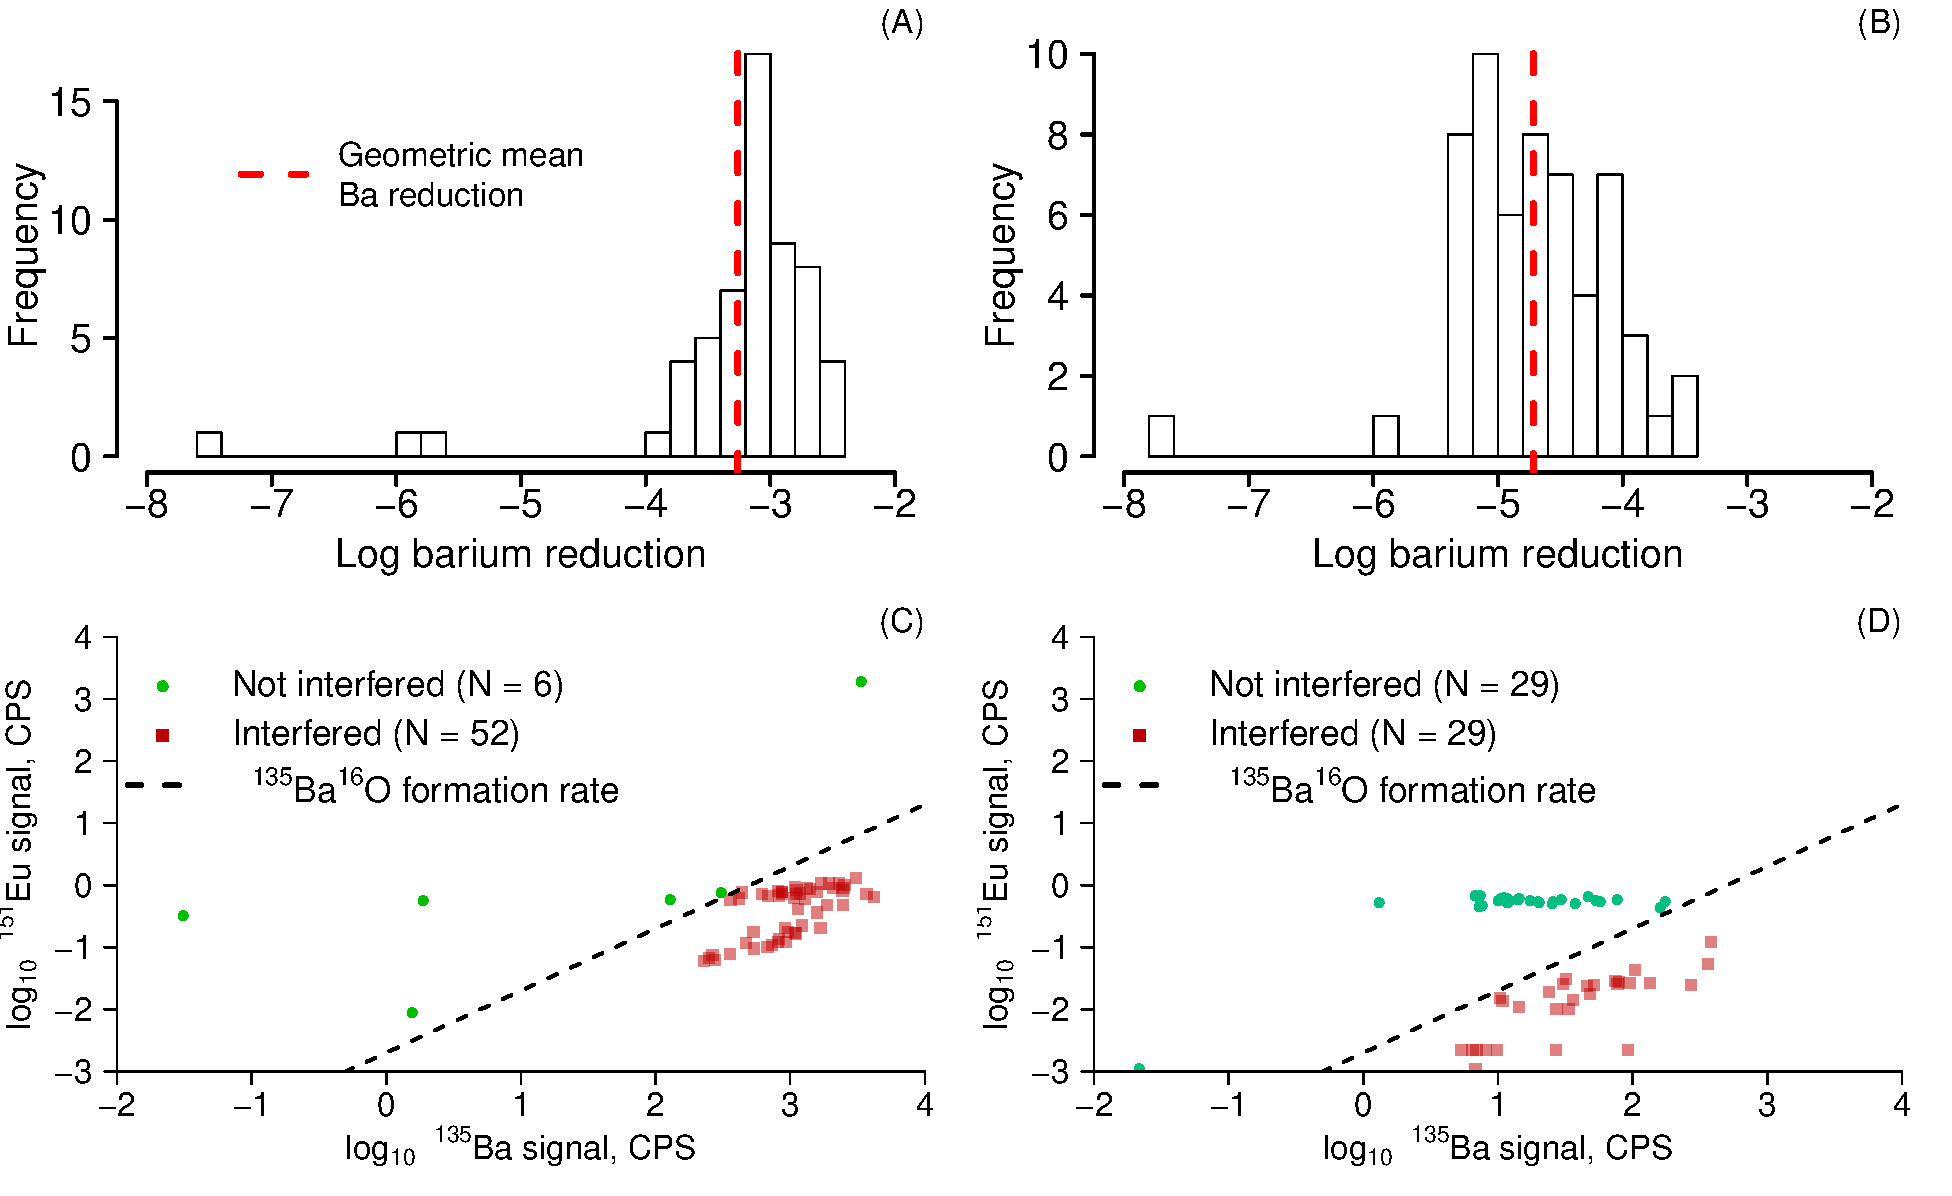
\includegraphics[width=0.8\textwidth]{Ch4_figures/Ba-removal.pdf}
\caption{Efficiency of Ba removal by LLE method (A, C) and ICP-MS octopole collision cell (B, D).
Results are for samples without (A, C) and with (B, D) \ce{H2SO4} addition to precipitate barite.
In (B) and (D), \ce{^{135}Ba^{16}O+} rate is inferred from 23 replicate analyses of a 200 ppb Ba standard after blank subtraction.
Interfered samples are those where accurate Eu determination could not be made due to excessive \ce{^{135}Ba^{16}O+} interference. In (D) the interfered samples were all unspiked experiments.}\label{fig:Ba-removal}
\label{default}
\end{center}
\end{figure}

Other experimental work in our shared lab space involves high concentrations ($\sim$mM) of Gd.
We ascribe the uniformly high Gd background in all experiments to cross contamination in this shared space.
In the ``Blank'' experiment (i.e. pH adjusted ASTM Type I water), all analytes were below detection (IDL $\sim$ 5 -- 20 ppt for 1\% false negative rate) except for Ba, La, and Gd. 
This indicates that the high La background could either be a result of laboratory cross-contamination (as with Gd) or an impurity in the organic phases used.
The latter supposition was investigated by direct contact of the mixed organic phases used (i.e. 3 mL 0.25 M HDEHP in heptane  + 1 mL octanol) with 4 mL of 6 N HCl, followed by analysis of the acid phase.
These results were below detection (not pictured), indicating no significant REE contamination of the organic phases.
While all chemicals were purchased at high purity, we can assume that the observed background concentrations in other experiments are due to trace contamination of these reagents.
Paradoxically, the level of these contaminations cannot be determined by ICP-MS without applying a separation/preconcentration technique such as the LLE method;
this makes source apportionment of the observed background concentration challenging.

\begin{sidewaysfigure}[htbp]
\begin{center}
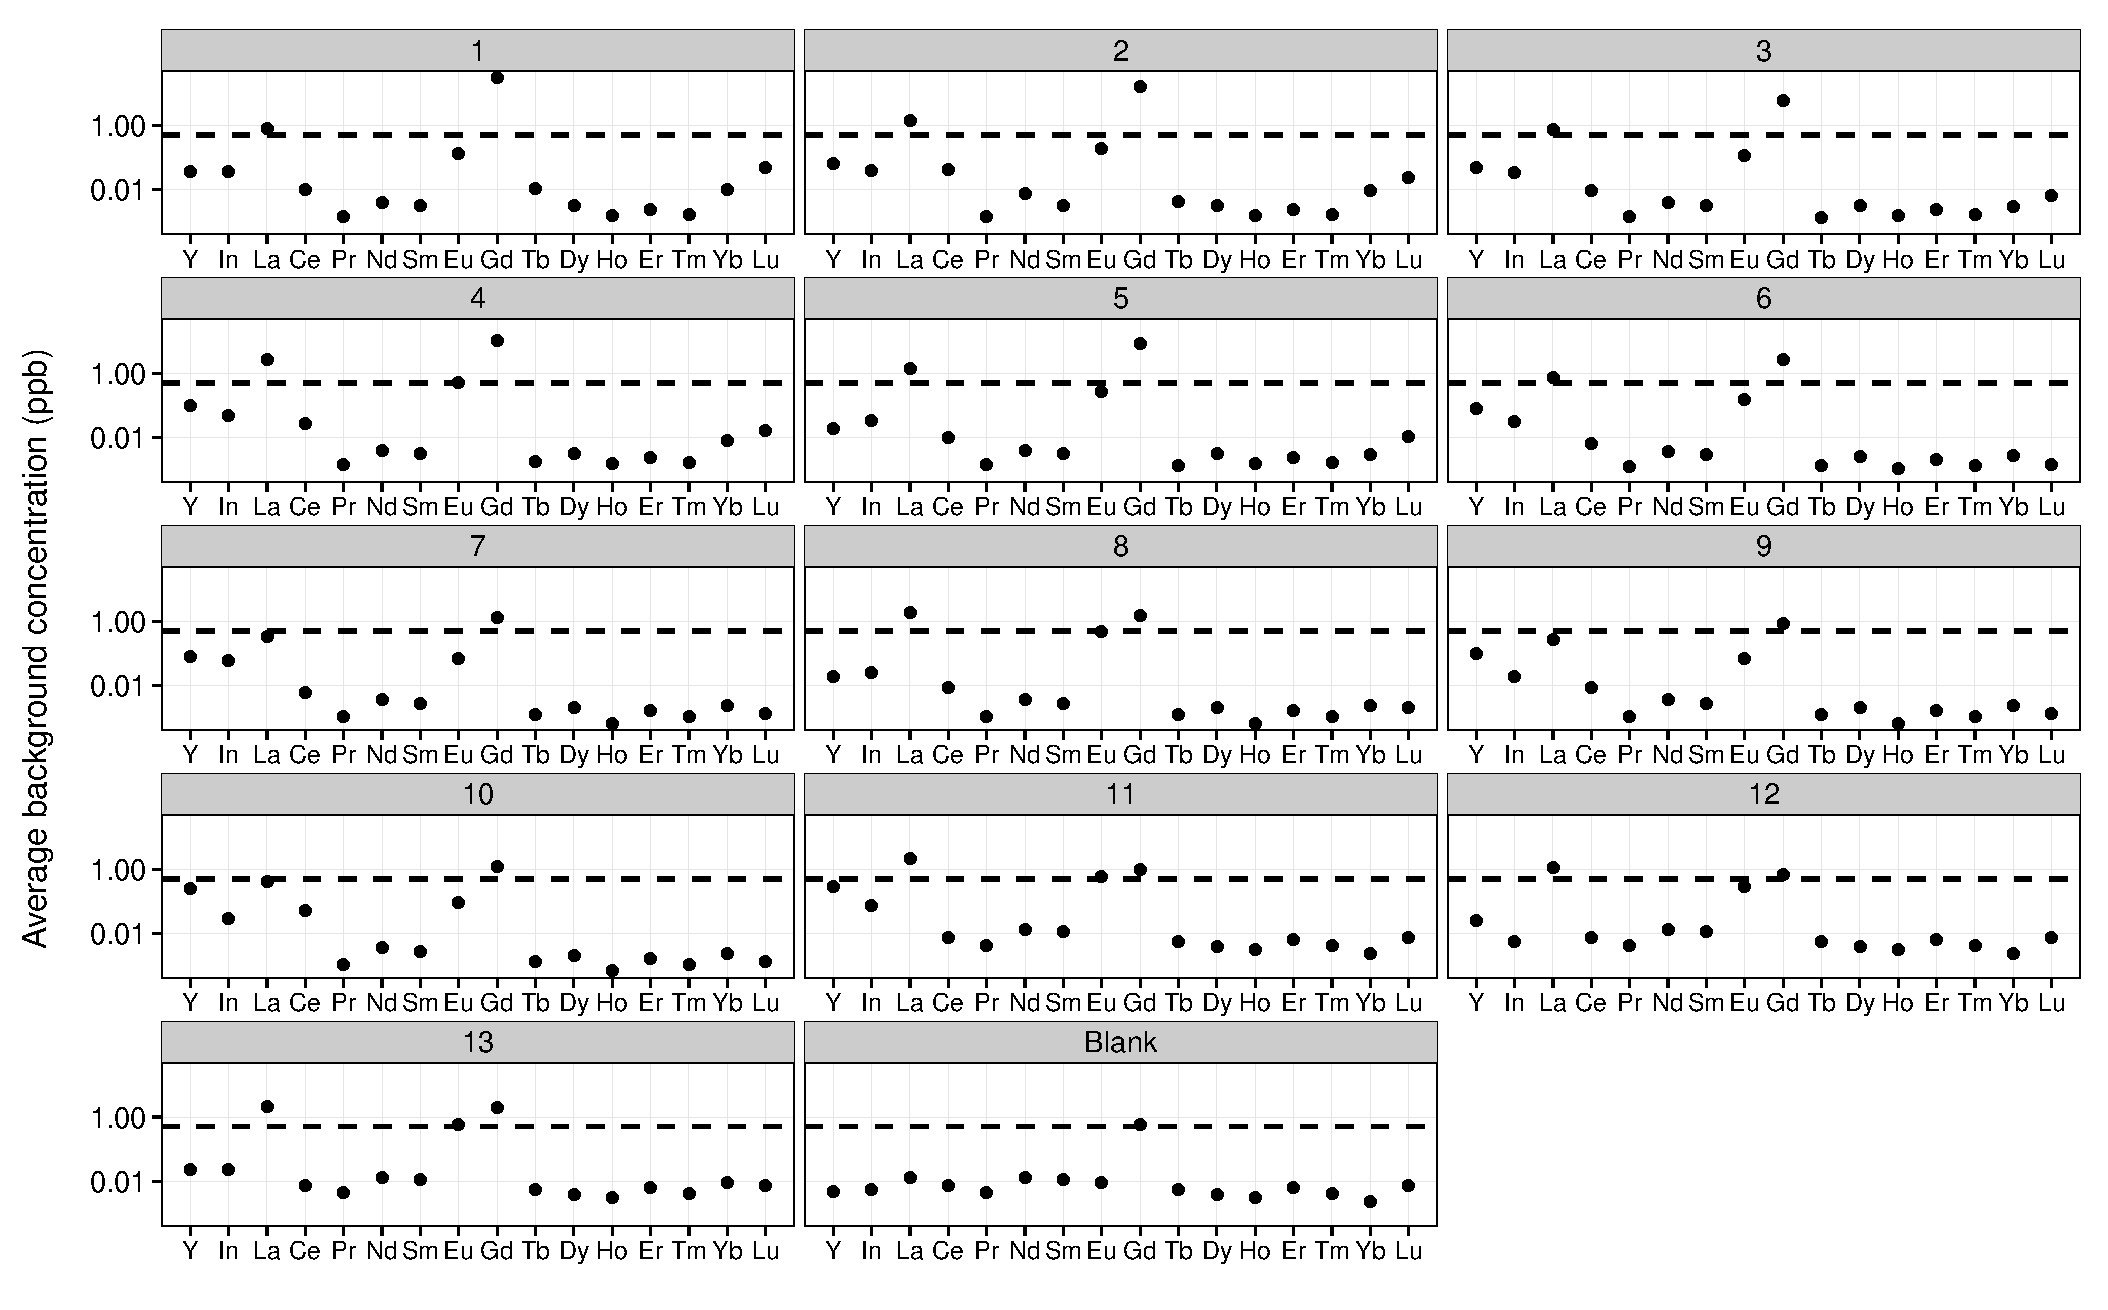
\includegraphics[width=0.95\textwidth]{Ch4_figures/REE-bkgd.pdf}
\caption{Average (from $n \geq 2$ replicates, except for Blank and experiments 6, 13) background concentrations of target analytes in samples without \ce{BaSO4} precipitation.
Dashed line at 500 ppt indicates the input concentration for all spiked samples.
Note that the y-axis is a logarithmic scale. Blank experiment represents pH adjusted ASTM Type I water.}\label{fig:REE-bkgd}
\end{center}
\end{sidewaysfigure}

\clearpage

\section{Doehlert experimental results}

These data represent the experiment and replicate ordered results of Doehlert matrix tests.
Each experiment number represents a unique set of solution conditions ([NaCl], [Fe], and [DOC]);
values for each of these parameters in each experiment is given in Table~\ref{tab:Doehlert}.

\begin{sidewaysfigure}[htbp]
\begin{center}
\includegraphics[width=\textwidth]{Ch4_figures/Exp-wise-LLE-recovery.pdf}
\caption{Elemental recovery in Doehlert matrix samples by LLE methodology (see Table~\ref{tab:Doehlert} for experimental conditions).
Recovery values for Eu were determined after dosing the LLE eluent with \ce{H2SO4} to precipitate barite;
all other recoveries were determined without barite precipitation.
Elements where the background concentration was determined to 250 ppt or greater (see Figure~\ref{fig:REE-bkgd}) were excluded (i.e. La and Gd in all experiments and Y in experiment 11).}
\label{fig:Doehlert-all}
\end{center}
\end{sidewaysfigure}



\end{appendix}

\bibliographystyle{unsrtnat}
\bibliography{proposal_bib}

\end{document}

